\documentclass[11pt,a4paper,twocolumn]{article}
\usepackage{amsmath}
\usepackage[numbers,sort&compress]{natbib}
\usepackage{url}
\usepackage{doi}
\usepackage{graphicx}
\usepackage{color}
\usepackage{ML}

\title{About the buckled shape}
\author{Martin Lind\'en,  \today} 
\date{} 
\begin{document}
\maketitle 
Here, we describe the buckled profile used for fitting an Euler
buckling profile to a set of points, with the main aim to explain the
various functions and their relations.

\begin{figure}
  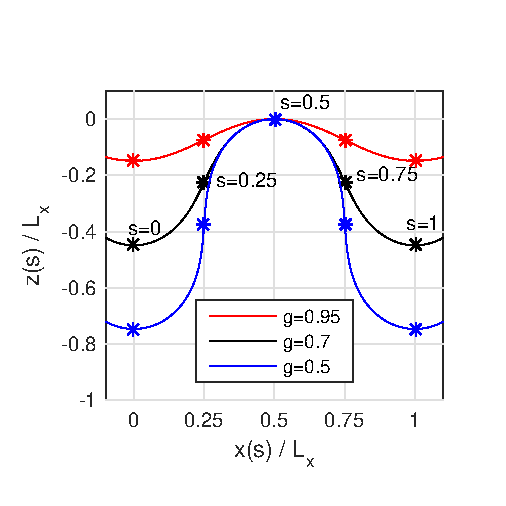
\includegraphics{figures/buckledshape.eps}
  \caption{\label{fig:buckle} The buckled shape in the $x,z$ plane for
    three different compression ratios $g=0.5,\;0.7,\;0.95$.}
\end{figure}
\paragraph{The buckled shape}
is handled by the function \texttt{buckleshape\_Fcoeff\_lin}, which
computes a parametric curve $x(s),z(s)$ (Fig.~\ref{fig:buckle}) and
some partial derivaties. The shape is parameterized by the projected
length $L_x$ and the compression ratio $g$, which are related to the
arc-length $L$ through
\begin{equation}
  g=\frac{L_x}{L},
\end{equation}
and related to the compression strain $\gamma$ used in
refs.~\cite{gomez2016,hu2013} via
\begin{equation}
  \lambda=\frac{L-L_x}{L}=1-g.
\end{equation}
This choice is practical when analysing buckling simulations, where
$L_x$ is kept fixed, but the arclength $L$ (and thus the dimensionless
$g$ as well) can fluctuate slightly during a simulation. The parameter
$s$ is proportional to an arclength parameter, so 
\begin{equation}
  \int_0^1\sqrt{\left(\frac{dX}{ds}\right)^2+\left(\frac{dZ}{ds}\right)^2}ds
  =L=\frac{L_x}{g}
\end{equation}
(although numerically, this is only true to about 3 decimal places).

The curvature along the buckled profile curve is given by
\begin{multline}
  C(s)=-\frac{\frac{dX}{ds}\frac{d^2Z}{ds^2}-\frac{dZ}{ds}\frac{d^2z}{ds^2}}{
    \left(
    \left(\frac{dX}{ds}\right)^2+\left(\frac{dZ}{ds}\right)^2
    \right)^{3/2}},
\end{multline}
where we use the convention that $C>0$ when the curve curves away from
the (upward-pointing) normal vector.

\texttt{buckleshape\_Fcoeff\_lin} uses an internal Fourier series
representation, so the cuves are periodic in $s$, with period 1. As
seen in Fig.~\ref{fig:buckle}, the curves are placed such that
\begin{equation}
x(0)=0,\quad
x(1)=L_x,\quad 
z(0.5)=0,
\end{equation}
and symmetry also dictates that $z(s)$ is symmetric, 
and $x(s)-s$ is antisymmetric,  around $s=0.5$:
\begin{equation}
  z(s)=z(1-s),\quad
  x(s)=L_x-x(1-s).
\end{equation}
Finally, $x(s)=sL_x$ at $s=0,0.25,0.5,0.75,1$.

The Fourier components used by \texttt{buckleshape\_Fcoeff\_lin} can
be recomputed using \texttt{buckleshape\_Fcoeff\_maketable}.

\paragraph{Fitting}
is done with the function \texttt{fit\_min2D\_buckle}, which solves a
non-liner least squares problem. Specifically, if the positions to be
fitted to are given by $x_i,z_i=1,2,\ldots$, the sum of squares
function is given by
\begin{multline}
    \chi=\sum_j
    \big(x_0+X(s_j,g;L_x)-x_j\big)^2\\
   +\big(z_0+Z(s_j,g;L_x)-z_j\big)^2,
\end{multline}
where both the translations $x_0,z_0$, the compression ratio $g$, and
the projected positions $s_j$ are fit parameters to be optimized.
\paragraph{Projecting:}
One the shape has been fitted, one might want to continue projecting
down points onto the buckled curve, for example to find out the
$s$-value of some molecule that was not used for fitting. This problem
is solved by \texttt{project\_min2D\_buckle}.

\bibliographystyle{unsrtnat} 
\bibliography{references}
\end{document}
